\section{Настройка программного комплекса SearchInform для поиска
конфиденциальной информации на основе подобия текстовых фрагментов }

\begin{figure}[H]
  \centering
  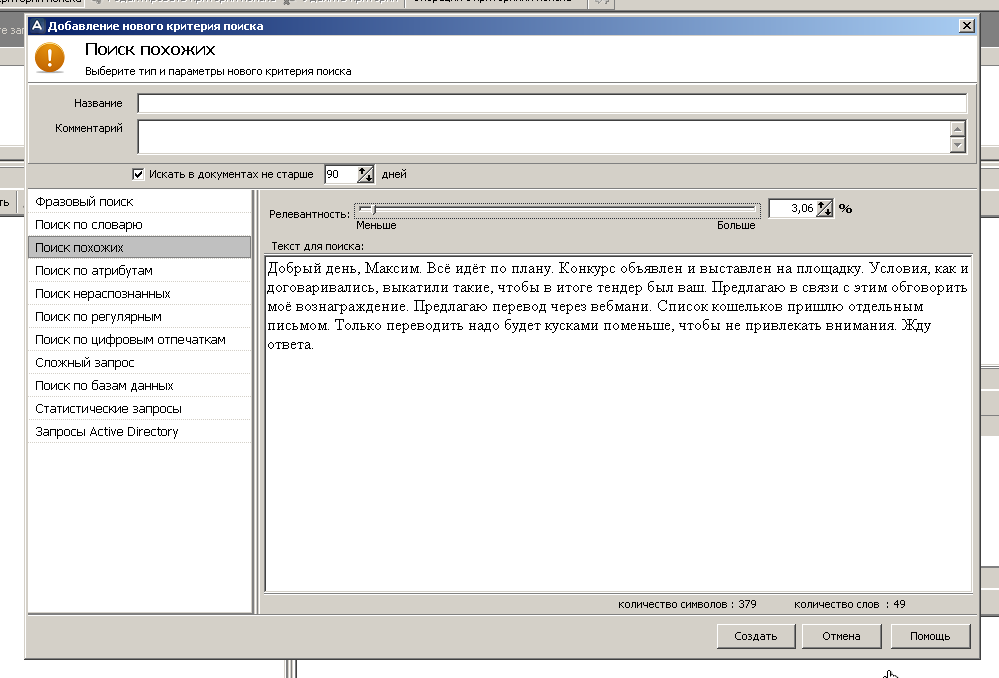
\includegraphics[width=\textwidth]{part4/1}
\end{figure}

\begin{figure}[H]
  \centering
  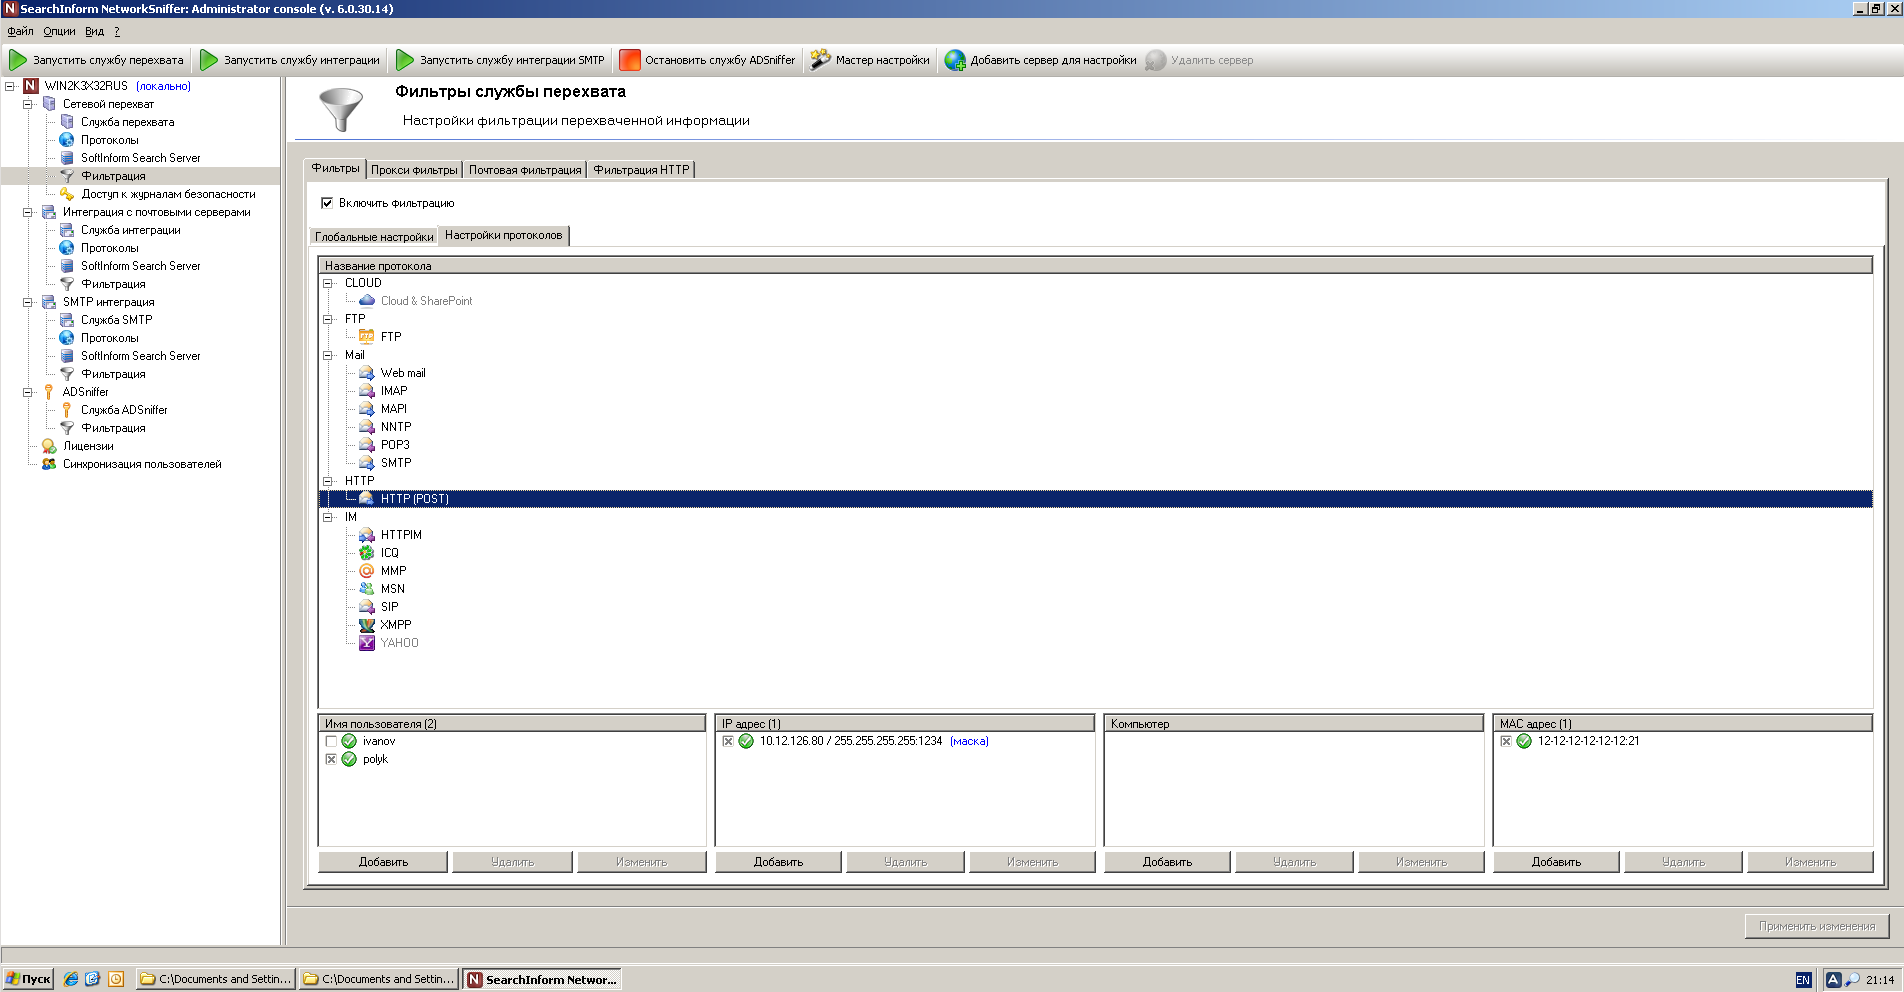
\includegraphics[width=\textwidth]{part4/2}
\end{figure}

\begin{figure}[H]
  \centering
  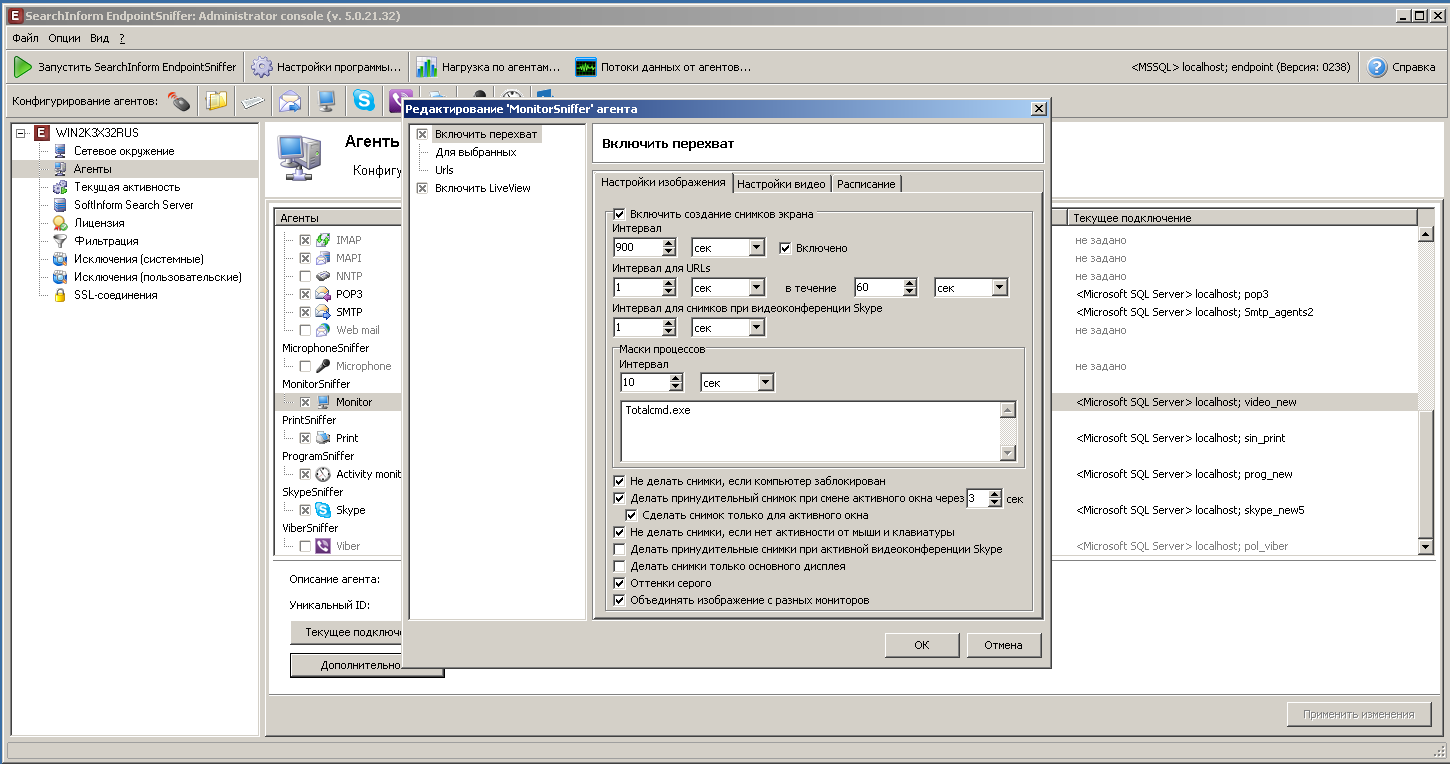
\includegraphics[width=\textwidth]{part4/3}
\end{figure}

\begin{figure}[H]
  \centering
  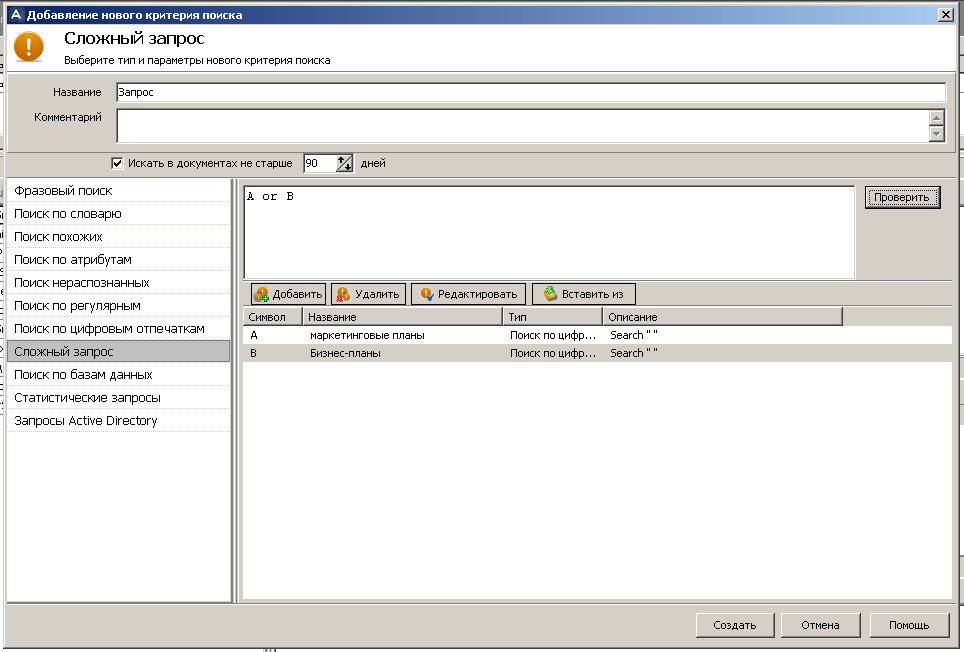
\includegraphics[width=\textwidth]{part4/4}
\end{figure}

\begin{figure}[H]
  \centering
  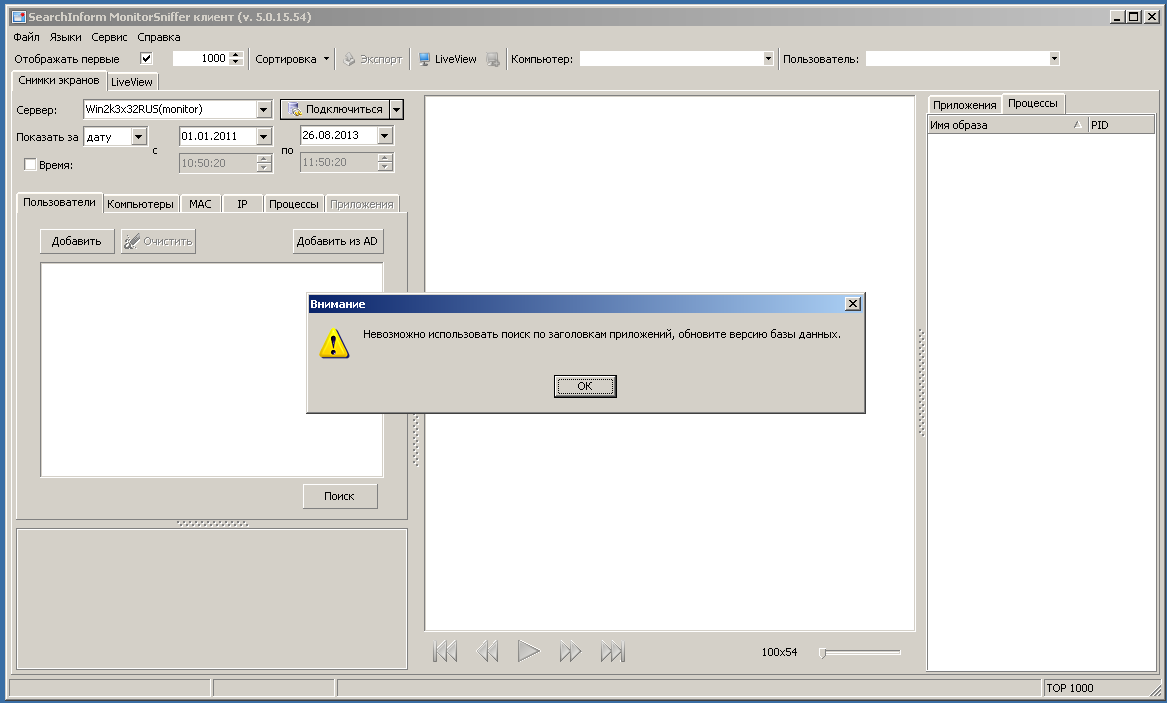
\includegraphics[width=\textwidth]{part4/5}
\end{figure}

\begin{figure}[H]
  \centering
  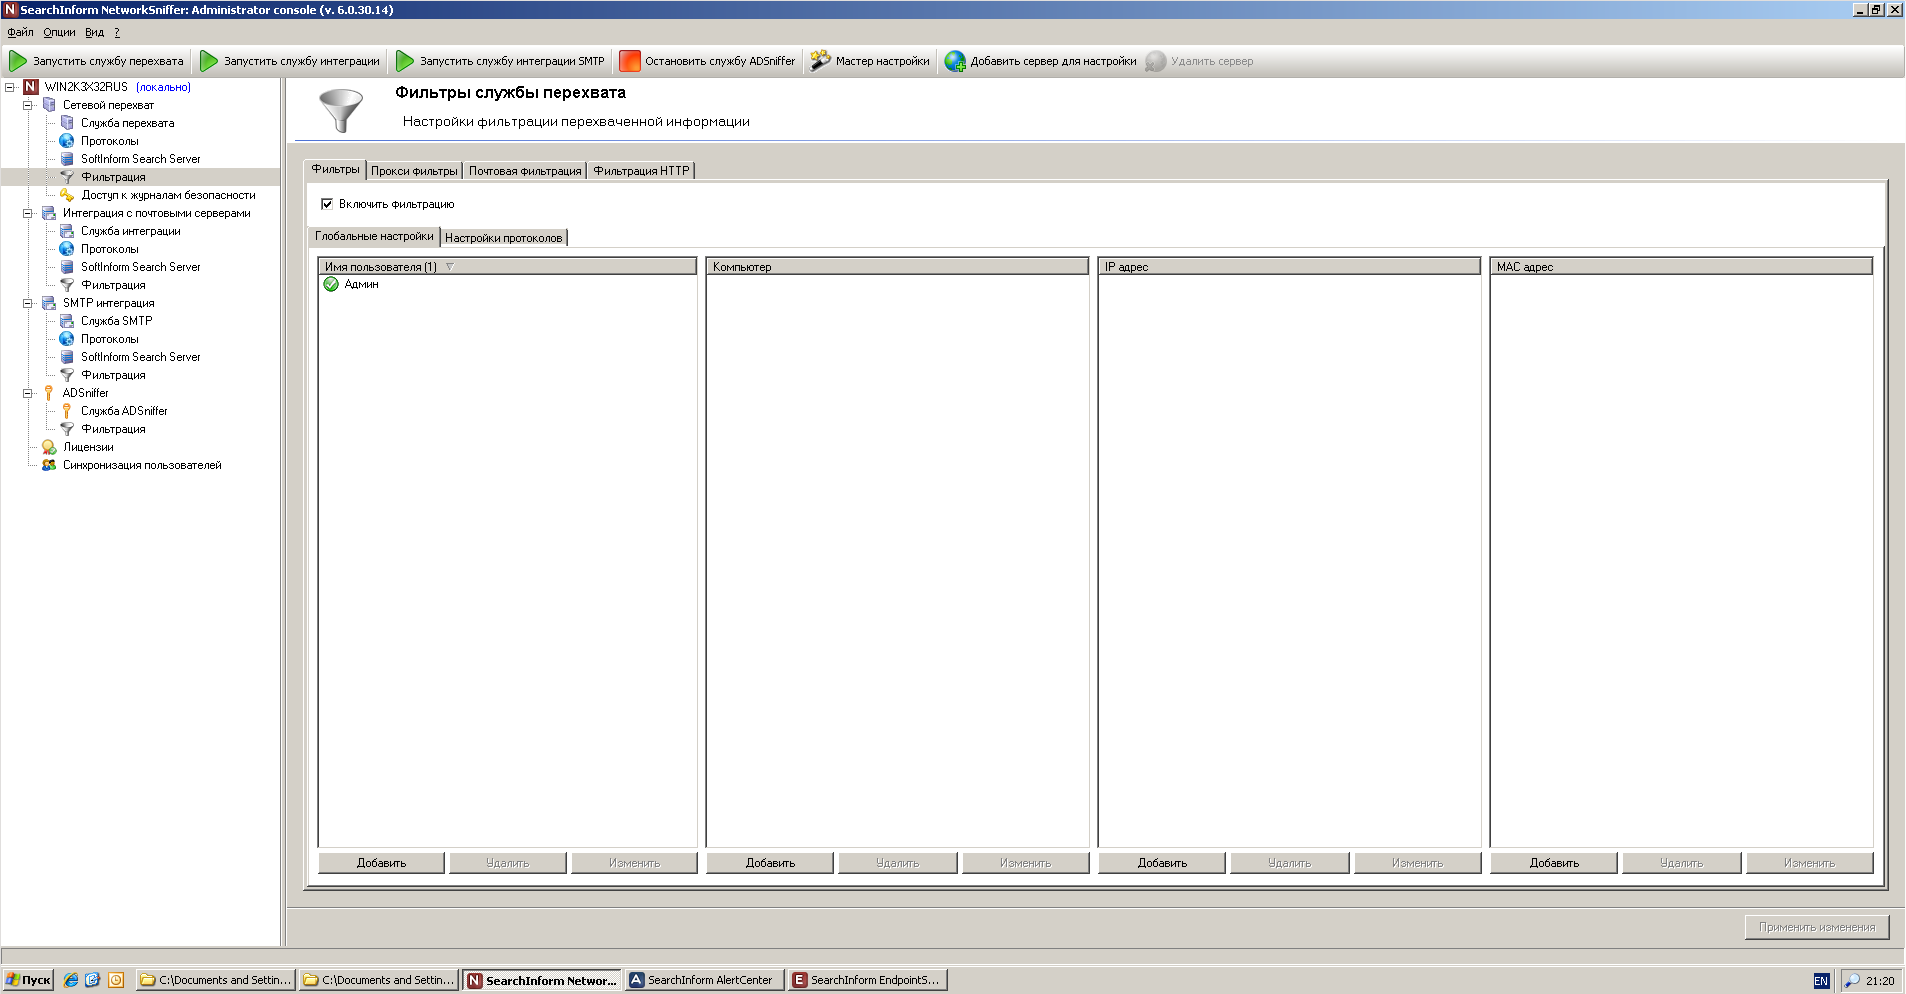
\includegraphics[width=\textwidth]{part4/6}
\end{figure}

\subsection{Контрольные вопросы}

\begin{itemize}
  \item Влияют ли пробелы между словами в запросе на результаты поиска по
    критерию «Поиск похожих»?

    Нет 

  \item Какие документы целесообразно искать с помощью критерия «Поиск
    похожих»?

    Небольшие текстовые файлы

  \item Какие документы целесообразно искать с помощью критерия «По цифровым
    отпечаткам»?

    Большие текстовые файлы

  \item Что значит оператор and?
    И
  \item Что значит оператор or?
    Или
  \item Что значит оператор not?
    Не
  \item Что такое стоп-слова? 
    Запрещенные подпоследовательности символов

  \item Как снять цифровой отпечаток из текста в графическом файле?
    Нужно как-либо факторизовать файл перед снятием отпечатка

  \item Можно ли снять цифровой отпечаток из pdf-файла?

    Нет, поскольку формат файла не содержит текст в явном виде, но можно
    распознать текст и работать отдельно с ним (потребует значительной
    вычислительной мощности)

  \item Можно ли снять цифровой отпечаток из java-файла? 

    Да

  \item Какие документы нецелесообразно искать с помощью критерия «По цифровым
    отпечаткам»? 

    Бинарные файлы

  \item Как объединяются простые запросы в сложные?
     
    С использованием логических конструкций

  \item Как проверить синтаксис сложного запроса? 

    Кнопка "Проверить"

\end{itemize}

